
% JuliaCon proceedings template
\documentclass{juliacon}
\setcounter{page}{1}
\usepackage{amsmath}

\begin{document}

% **************GENERATED FILE, DO NOT EDIT**************

\title{Locality-Aware Message Passing with ArrayChannels.jl}

\author[1]{Rohan McLure}
\author[1]{Josh Milthorpe}
\affil[1]{Research School of Computer Science, Australian National University, Canberra}

\keywords{Distributed, Access Locality, HPC}



\maketitle

\begin{abstract}
Performance outcomes for numerical codes involving large data
manipulation depend on efficient access of memory. We introduce the ArrayChannels.jl library for
manipulation of distributed array data with considerations for cache
utilisation patterns. In contrast to communication constructs
implemented by Julia's remotecall, communication in
the library occur entirely in-place, improving temporal locality. We evaluate the
performance of ArrayChannels.jl constructs relative to
comparable MPI and Distributed.jl implementations of the Intel
PRK, yielding improvements of up to 150\%.
\end{abstract}

\section{Introduction}
The Julia language offers many conveniences to the development of
numerical codes that are geared towards performance. Julia favours rapid
prototyping by adopting a highly optimised \textit{JIT} compilation approach to
program execution, as well as the convenience of dynamic dispatch for
user-made functions. The implicit vectorisation of codes massively
accelerates the performance of user-defined array access codes.

The suitability of the language for HPC applications will nonetheless
continue to hang on the ability of programmers to deliver strong
parallel performance with relative ease. Throughout this article, the
particular form of parallelism that we refer to is distributed
computing. While multiprocessors provide a high degree of parallelism, distributed clusters can provide extremely high performance scalability. Targeting many-core systems can serve to increase the impact of the Julia language for HPC.

We produce the \texttt{ArrayChannels.jl} library, covering a variety of
parallelism patterns operating on arrays in a distributed computing
context, all while guaranteeing the programmer improved access locality
over default Julia constructs. Much like how a \texttt{RemoteChannel} will reference a channel residing at a particular process, \texttt{ArrayChannel} constructs reference persistent data buffers to facilitate cache-aware communication.
All communication primitives between these
constructs occur synchronously and in-place. In-place communication
causes the manipulation of message contents following arrival to be more
efficient by increasing cache locality and so reducing the impact of
memory latency. We briefly discuss the ramifications of access locality in
\S~\ref{sec:access-locality}

We evaluate the performance outcomes of using \texttt{ArrayChannels.jl}
relative to the Julia \texttt{Distributed.jl} library and
equivalent MPI constructs. We use a subset of the Intel
Parallel Research Kernels to obtain performance readings for both
many-core and many-node trials on HPC hardware.

In addition to performance benefits, in \S~\ref{sec:arraychannels}
we demonstrate how \texttt{ArrayChannels.jl} may be used to effectively
generate distributed codes concerning array-manipulation with a higher
degree of productivity than current Julia primitives.


\section{Background}
Here we discuss the underlying mechanisms that lead to differences in
distributed performance outcomes between \texttt{ArrayChannels.jl} and
\texttt{Distributed.jl}, and provide a brief introduction to our
evaluation benchmarks. The mechanisms that we refer to involve access
locality for processor caches, as well as discussion on the various
modes of message passing in distributed environments.

We discuss our evaluation benchmarks, including a subset of the Intel
Parallel Research Kernels.

\subsection{Access Locality}
\label{sec:access-locality}

Access locality \cite{patterns} refers to the likelihood for memory access patterns to target the same or adjacent memory regions repeatedly during execution. We describe two aspects of access locality: temporal and spatial locality. Temporal locality refers to the proximity in terms of timing of multiple accesses to the same memory region, while spatial locality
refers to the proximity in terms of location of relevant data entries to one another in memory.

\subsubsection{Temporal Locality}
\label{sec:temporal-locality}

Essentially, temporal locality in part determines the maximum amount of
time for which program data may remain at readily-accessible regions of
the memory hierarchy. When a greater proportion of the computational
effort can be performed on data currently residing in processor cache,
the total effect of memory latency is mitigated. Alternatively, poor
temporal locality can lead to \emph{cache misses}, scenarios where cache
is prematurely flushed, and program data must be re-fetched prior to use,
leading to more memory latency. Intuitively, programmers will wish to
ensure when possible that data structures under perpetual use within the
program remain within processor cache, so that all modifications to this
data may incur less overhead. In \S~\ref{sec:arraychannels}, we
discuss how in a message-passing context, how retaining a single message
buffer for repeat communication events can lead to improved parallel
performance.

\subsubsection{Spatial Locality}
\label{sec:spatial-locality}

Spatial locality represents the condition whereby relevant program data is situated close-by in memory. Higher spatial locality increases the effectiveness of cache pre-fetching, as a larger proportion of cache lines will contain the necessary program data. Spatial locality can be improved by storing program data contiguously in memory. While array representations provide a high degree of spatial locality, programmers
must be aware of the effects of striding on multidimensional arrays.

\subsection{Message Passing Models}
\label{sec:message-passing}

Message passing provides a mode for both synchronisation and the
communication of data between processes in a parallel computation. This
methodology is particularly useful when there is no notion of shared
memory between processes, as in the case of distributed computing. Julia
implements message passing through its \texttt{Distributed.jl} module in
the standard library. The two main primitives available to the user are the
\texttt{remotecall}, as well as \texttt{Future} objects. Processes may message
one another by means of a remote procedure call, whereby arguments to
the remote call and other captured variables are communicated to the
recipient process. A \texttt{Future} fulfils the synchronising role of
a remote call, encapsulating the completion state of function in
execution at another process.

A combination of these two primitives form the \texttt{RemoteChannel},
which is a sort of handle to a \texttt{Channel} construct appearing at
another worker process. While a \texttt{RemoteChannel} may provide both
synchronous and asynchronous communication, both forms will invoke an
eager communication model. We provide a description of two different
modes of point-to-point message passing in play in both
\texttt{Distributed.jl} and \texttt{ArrayChannels.jl}.

\subsubsection{Eager Communication}
\label{sec:eager}

In eager message passing, processes will immediately attempt to send
messages \cite{illinois, ompi}, without needing to first wait for the
approval of the recipient process. Eager message passing permits expensive
communication operations to be initiated prior to the arrival of a
`ready to receive' notification. In various MPI implementations such as
OpenMPI, this is facilitated by the short message protocol, which causes
the message to be copied to the output buffer when specified by the
receive notification. In the case of Julia, this memory copy is not
required, as each message that arrives will have a new output buffer
allocated for immediate use.

\begin{figure}[htb]
	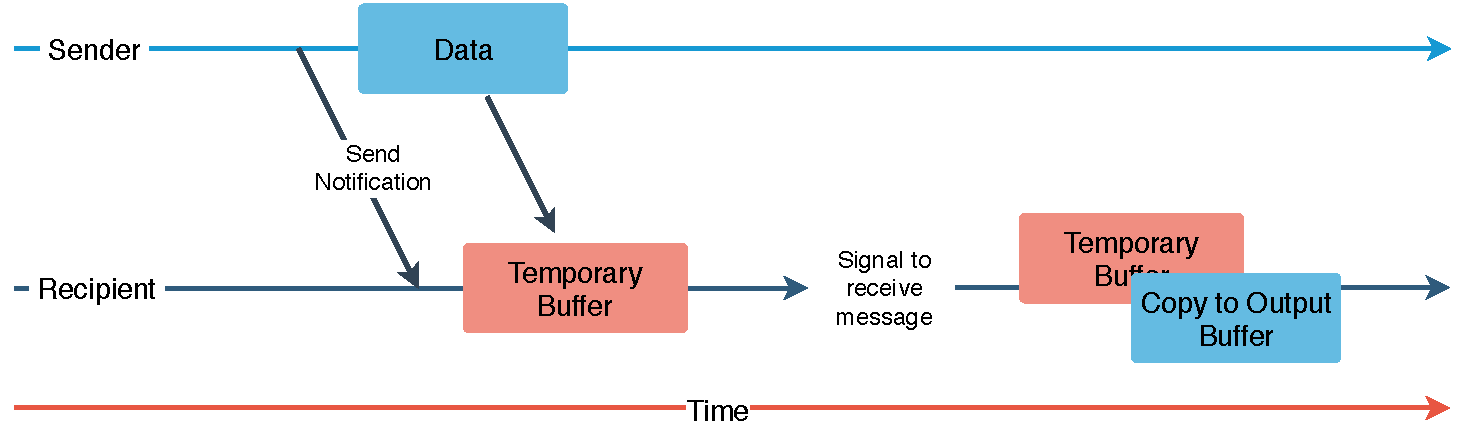
\includegraphics[width=\linewidth]{figs/Eager.pdf}
	\caption{The eager communication model}
	\label{fig:eager}
\end{figure}

The \texttt{Distributed.jl} framework causes messages to be sent in an
eager manner, even on synchronous channel constructs. While access to a
\texttt{RemoteChannel} may be synchronised, any attempt to \texttt{put!}
(or initiate sending) a reference type will fully transfer the
referenced data, but only depositing the reference pointer in the
recipient's channel when it is signalled as able to do so. In
\S~\ref{sec:transpose-results}, we discuss how eager message
passing can provide performance advantages under pathological examples.

\subsubsection{Rendezvous Communication}
\label{sec:rendezvous}

Rendezvous communication involves both sender and recipient
synchronising over either mutual acknowledgement of messaging, or on the
completion of the data transfer \cite{illinois, ompi}. In the rendezvous
mode, data will not begin to be transferred until both sender and
receiver have each confirmed by means of a handshake their intent to
begin. While rendezvous communication requires that message transfer
occur at a particular time (namely, following a successful handshake),
the receiving process may offer in their intention to receive a preferred
buffer which may be written to directly after synchronisation. In this
way, rendezvous message passing may be used to avoid an extraneous
memory copy, at the cost of additional synchronisation. While frameworks such as \texttt{Distributed.jl} that utilise eager message passing may omit the memory copy step, this mode will reduced temporal locality, as new buffers must be selected between communication events.

\begin{figure}[htb]
	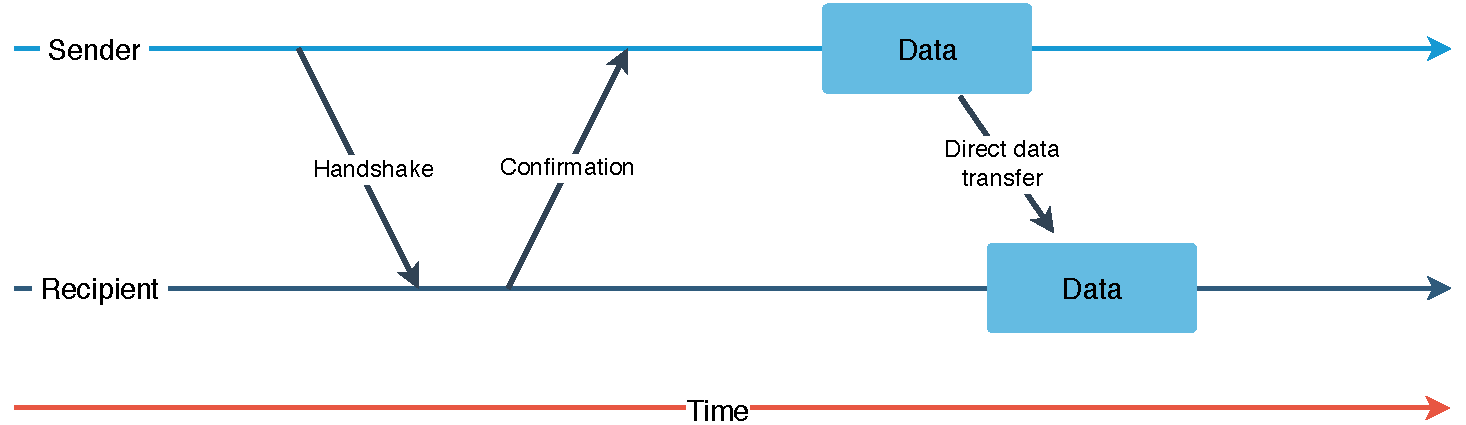
\includegraphics[width=\linewidth]{figs/Rendezvous.pdf}
	\caption{The rendezvous communication model}
	\label{fig:rendezvous}
\end{figure}

An \texttt{ArrayChannel} construct will require rendezvous message
passing to ensure that the same output buffer is used for each
successive communication instance. We discuss how the differences
between these two modes affect the behaviour of the
\texttt{ArrayChannels.jl} library in \S~\ref{sec:arraychannels}.

\subsection{Evaluation Techniques}
\label{sec:eval}

To evaluate differing performance outcomes between
\texttt{Distributed.jl} and \texttt{ArrayChannels.jl} communication
nodes, we provide performance comparison on a series of benchmarks. For
an analysis of maximum obtainable data-transfer rate, we provide the
results of a two-process ping-pong benchmark. As a projection of
performance outcomes on more realistic use cases, we compare performance
readings on a subset of the Intel Parallel Research Kernels, providing
readings for a variety of core-counts to indicate the effect of
\texttt{ArrayChannels.jl} communication primitives on scalability. Our
scalability results are given in terms of weak-scaling, whereby problem
size increases roughly linearly with core-count, to enable each parallel
entity to operate on the same amount of local data.

\subsubsection{Intel Parallel Research Kernels}
\label{sec:intel-prk}

The Intel PRK~\cite{Wijngaart} are a series of HPC
kernels that serve to predict the performance of parallel environments
and frameworks for realistic computation tasks.

We provide performance measurements on three of these kernels, namely
Reduce, Transpose and Stencil, due to their emphasis on array computing
which is a strength of the Julia language. Moreover, these kernels
represent real data-parallelism workloads, which are commonplace in the
numerical computing applications of the language.

\subsubsection{The Reduce Kernel}

The reduce kernel reduces a series of large vectors by accumulating
their vector sum into an output vector at each iteration. For each
additional core provided to the kernel, two vectors of equal size are
provided so as to provide each core with some local computation.

\begin{figure}[htb]
	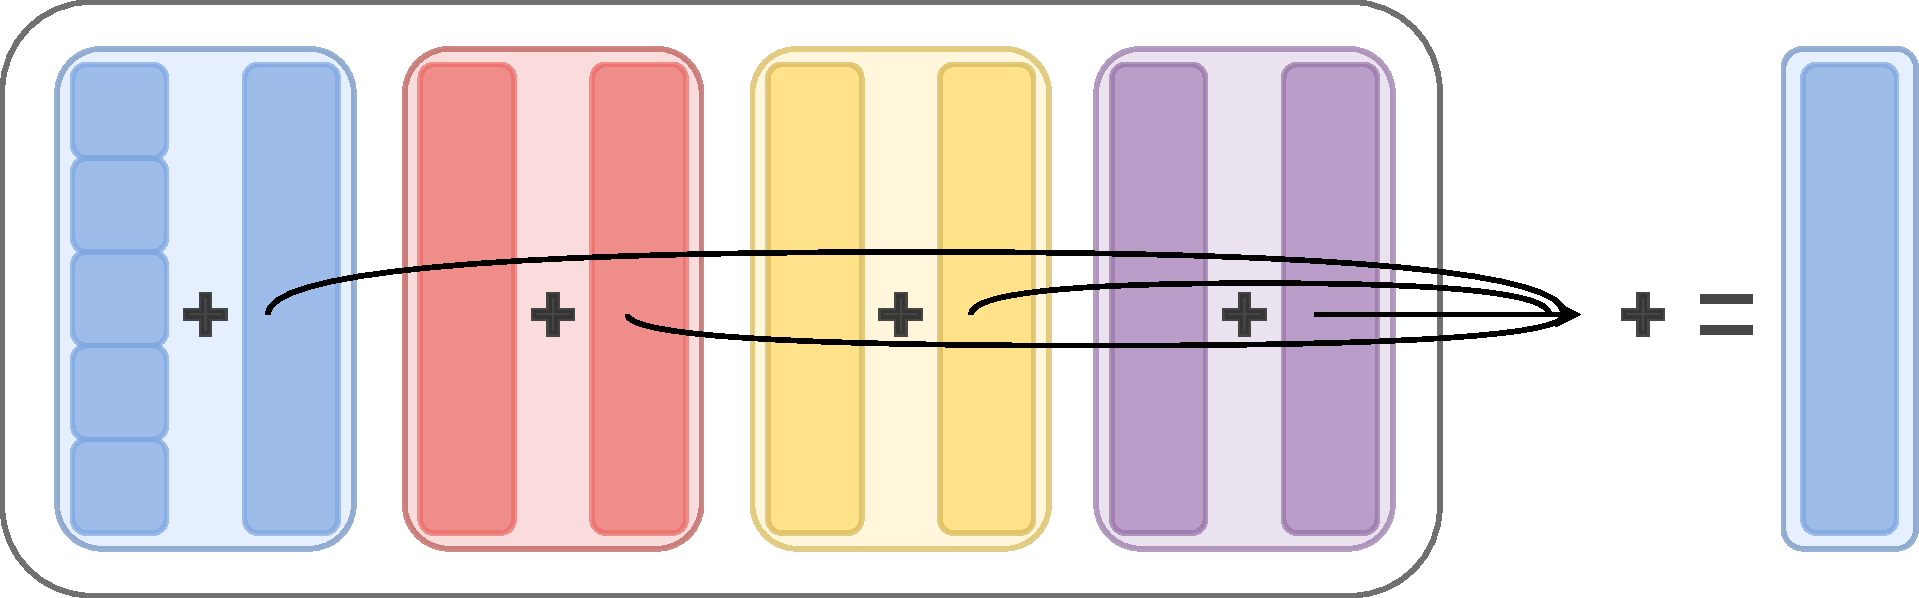
\includegraphics[width=\linewidth]{figs/Reduce.pdf}
	\caption{Distributed reduce kernel}
	\label{fig:reduce-diagram}
\end{figure}

In a distributed context, this is accomplished by allocating two large
vectors at each locale, computing the local sum and then performing a
distributed reduction on the resultant vector. In figure~\ref{fig:reduce-diagram}, reduction occurs in stages occuring at different compute nodes for improved parallelism. In MPI, this is
facilitated directly by the \texttt{MPI\_Reduce} directive, which
causes the MPI runtime to conduct the parallel reduction with a single
destination rank using whichever topology it deems most suitable. As the
MPI Reduce implementation performs its work in place, our equivalent
implementations in Julia attempt to duplicate this behaviour by
implementing the tree topology using point-to-point communication. In
\S~\ref{sec:reduce} we comment on the utility of language
directives for directly addressing parallelism patterns.

\subsubsection{The Transpose Kernel}
\label{sec:transpose-kernel}

The transpose kernel will at each iteration transform the memory
representation of a dense matrix so that columns are stored in the row
format and vice versa. In a distributed context, where the matrix is
fragmented among different locales, the transpose of a pair of indices
may belong to a different locale, and as such data communication is
required. In practise, the matrices are distributed into "column
blocks", with one column block given to each process. Figure~\ref{fig:transpose-diagram} demonstrates how off-diagonal regions of
column blocks must be communicated with other processes at each
iteration. The colours represent the distribution of data between workers.
Arrows connecting differently-coloured regions indicate that communication must occur between the owners of the regions.

\begin{figure}[htb]
	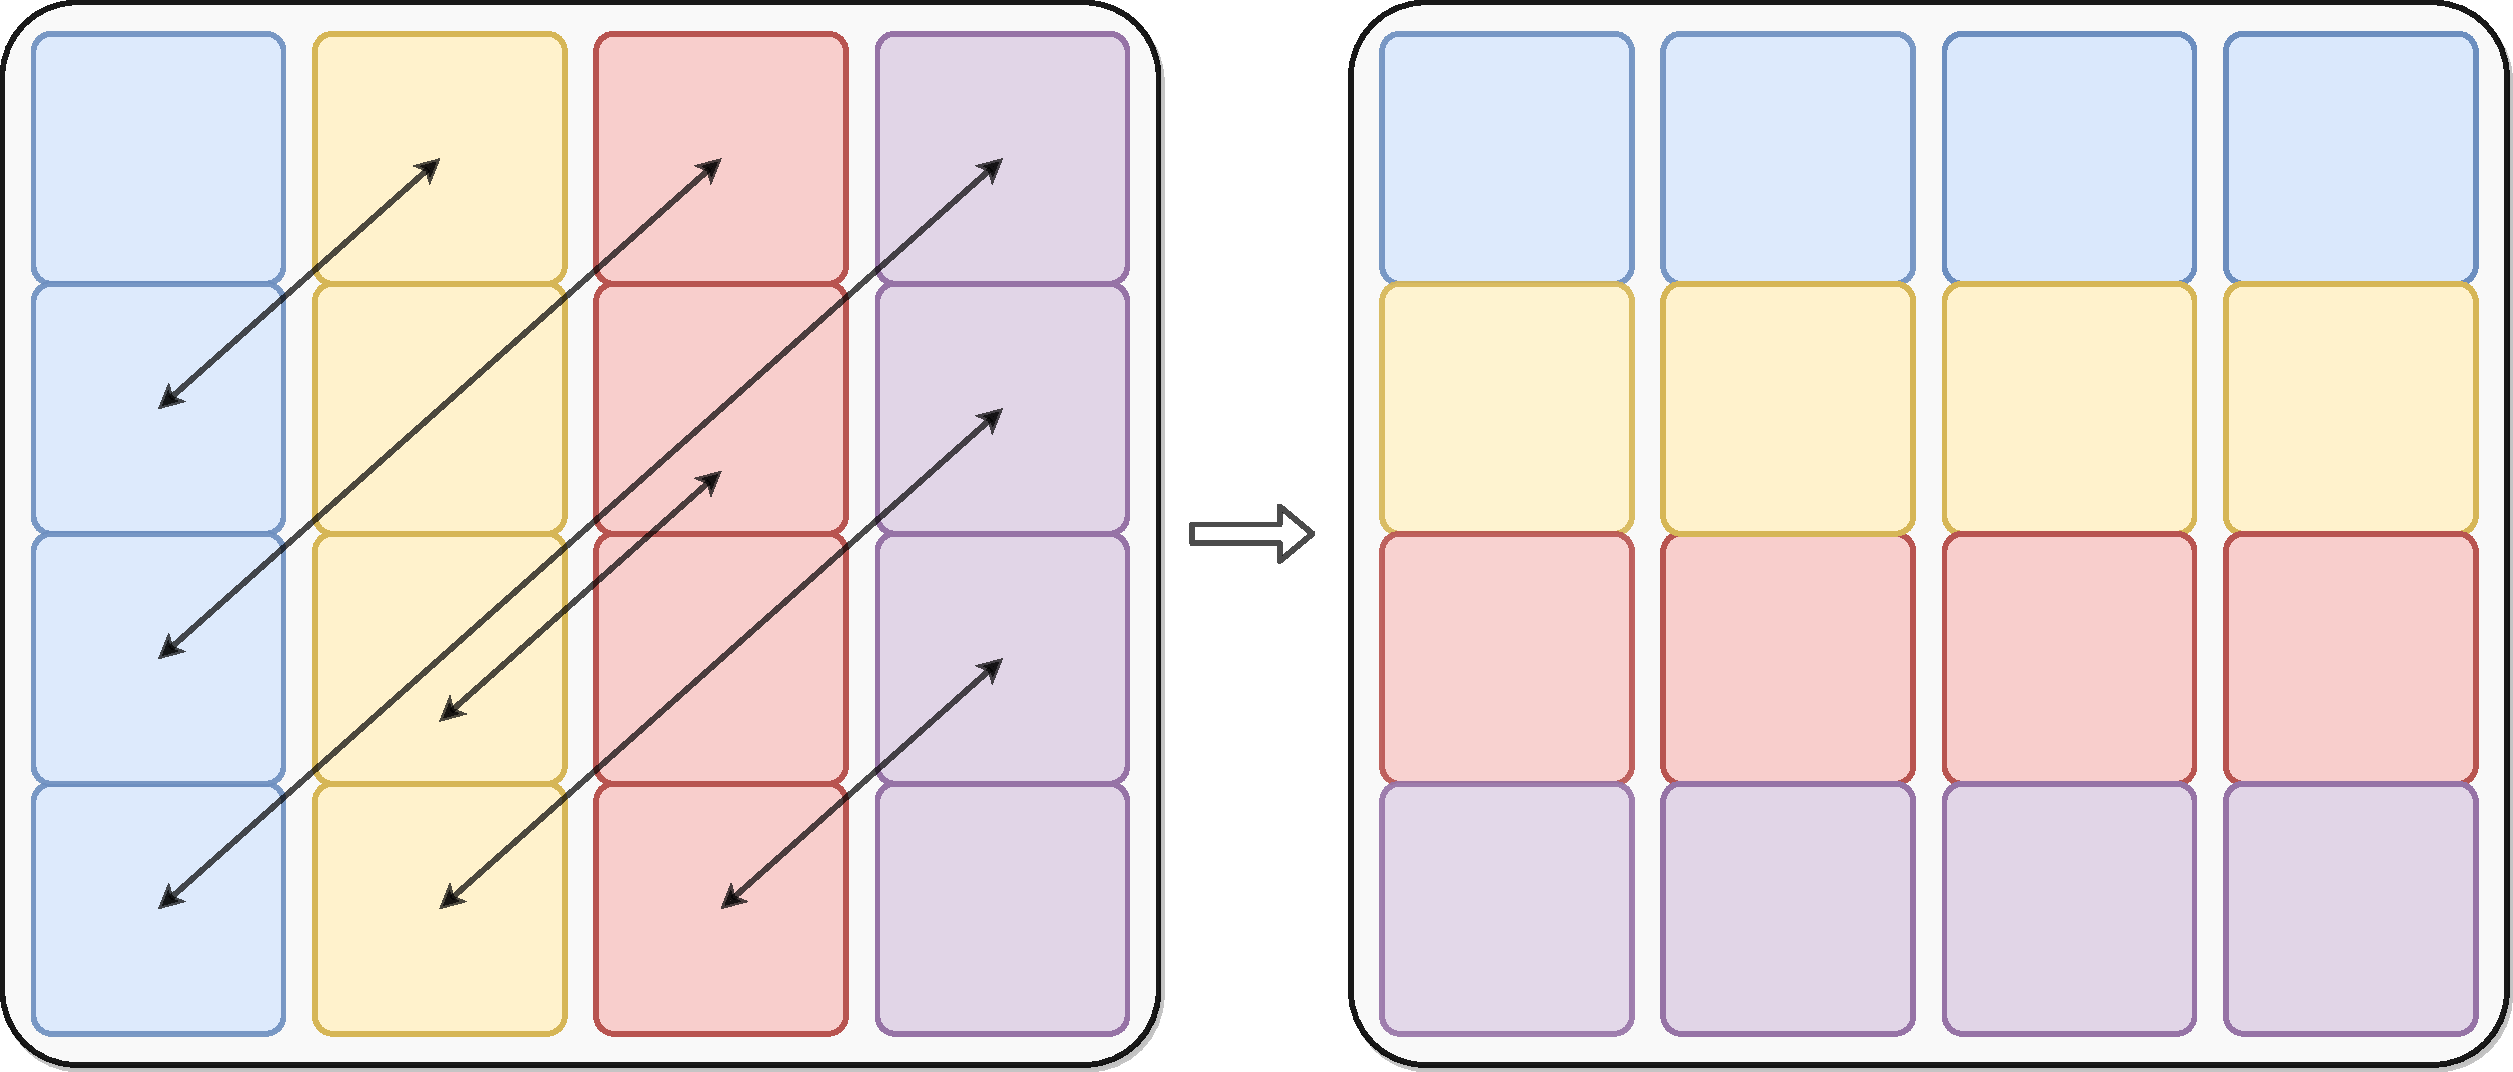
\includegraphics[width=\linewidth]{figs/Transpose.pdf}
	\caption{Distributed transpose kernel}
	\label{fig:transpose-diagram}
\end{figure}

At each iteration, the total amount of data that must be communicated
increases quadratically with the order of the matrix, and each worker
must communicate with every other worker. This kernel provides an
intense stress on the efficiency of the communication model, while
providing minimal arithmetic intensity.

\subsubsection{The Stencil Kernel}

The stencil kernel involves repeatedly applying a point-wise operator to
each element of a dense matrix, where the point-wise operator depends on
the value of neighbouring data points. For a distributed context, this
kernel may be parallelised by decomposing the source matrix into square
blocks and distributing each block to a different worker process.
Applying the stencil operator to indices that border the divisions will
require the acquisition of data from neighbouring processes, as depicted
in figure~\ref{fig:stencil-diagram}. In the diagram, colours are used to represent the distribution of matrix data, and green subregions represent the communication boundaries.

\begin{figure}[htb]
	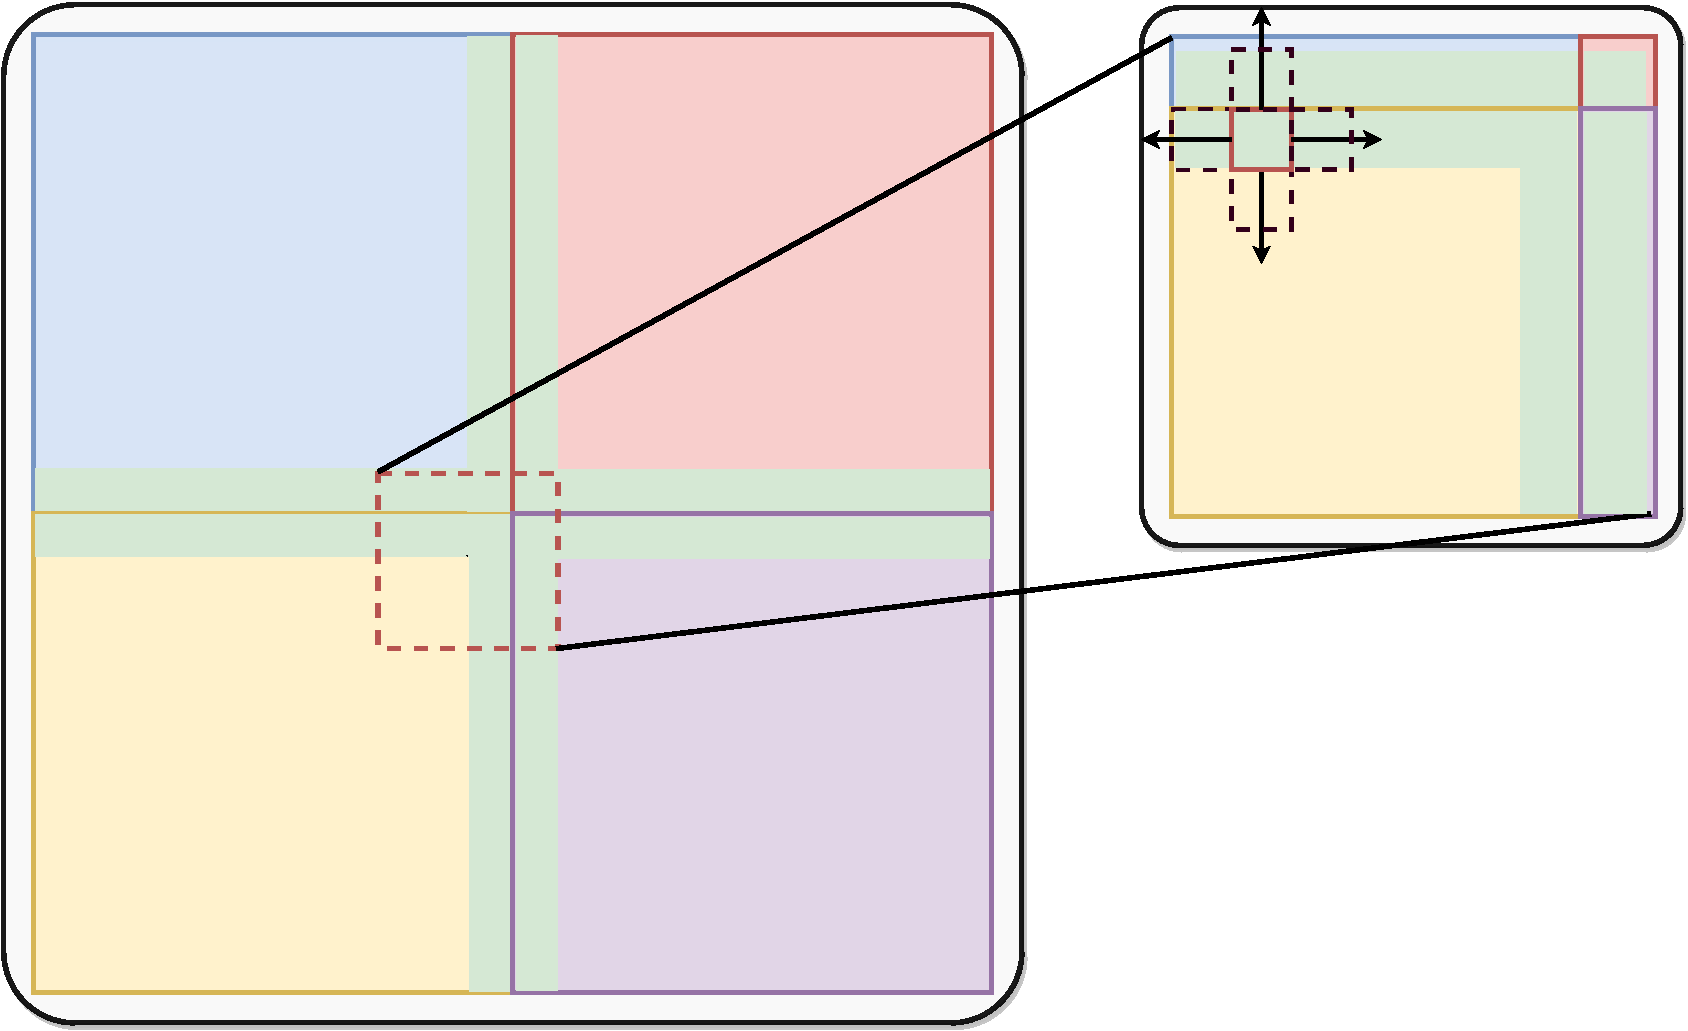
\includegraphics[width=\linewidth]{figs/Stencil.pdf}
	\caption{Distributed stencil kernel}
	\label{fig:stencil-diagram}
\end{figure}

The regions of data dependencies that lie on the borders between locales
are known as "ghost regions". A parameter known as the "stencil radius"
determines the width of these ghost regions, and so total amount of data
to be communicated increases linearly with respect to the order of the
matrix. Unlike the transpose kernel, the stencil kernel requires the
communication of only relatively small amounts of data, while providing
a high arithmetic intensity.

\section{The ArrayChannels.jl Library}
\label{sec:arraychannels}

The \texttt{ArrayChannels.jl} library provides synchronous, in-place
communication options for message passing, utilising rendezvous message
passing. This is achieved by providing an \texttt{ArrayChannel}
construct encapsulating a template for the forms of array communication
that must occur. Constructing an \texttt{ArrayChannel} will require
specification of the processes that must participate in relevant
communication events. Each participating process will allocate a buffer
of the same fixed size that will be reused for all communication tasks.

In distributed computation tasks that depend on data to be received as
messages from other processes, reuse of the same message buffers
improves temporal locality. This in turn causes the receiving of new
messages and actions upon message contents to be more likely to occur in
cache and with fewer cache misses.

\subsection{Point-to-Point}
\label{sec:p2p}

For point-to-point communication, we provide two commands, \texttt{put!}
and \texttt{take!}, which allows processes to send messages to, or receive
from, a specified process. In code snippet~\ref{code:put-take}, \textbf{process
1} creates an \texttt{ArrayChannel} to facilitate communication between
worker processes. By using a remote call, the programmer may initiate
communication by passing the \texttt{ArrayChannel} as arguments to an invocation of either
\texttt{put!} and \texttt{take!}. \texttt{ArrayChannel} constructs associate with different
data buffers depending on which process interacts with the reference.

\begin{figure}[htb]
	\begin{lstlisting}[language=Julia]
# 10 x 10 buffer
AC = ArrayChannel(Float64, workers(), 10, 10)

@sync begin
	@spawnat 2 begin
		fill!(AC, 1.0)
		put!(AC, 3)
	end
	@spawnat 3 begin
		take!(AC, 2)
		@assert AC[1,1] = 1.0
	end
end
	\end{lstlisting}
	\caption{Message of 10 x 10 matrix of ones sent via point-to-point messaging}
	\label{code:put-take}
\end{figure}

\texttt{put!} and \texttt{take!} operations will block until all buffer
contents have been communicated and written at the recipient's buffer.
\texttt{ArrayChannels.jl} will then
simply take the contents of the input buffer and deposit them in the
output buffer at the recipient process, using the same buffer for each
successive communication operation for improved temporal locality.

\subsection{Reduction}
\label{sec:reduce}

All participants in the underlying \texttt{ArrayChannel} must signal
their intent on initiating a reduction by calling \texttt{reduce!} on
the remote channel reference, supplying the reduction operator and
`root' process which will receive the resultant data. In figure~\ref{code:reduce}, the master process initialises an
\texttt{ArrayChannel} for the worker processes, and then causes each
participating process to signal for a sum reduction on their local data,
directing the result towards \textbf{process 2}. After this reduction has taken
place, only \textbf{process 2}'s data will be modified. \texttt{reduce!} will
block so long as the calling process is still required to facilitate the
reduction under the current topology.

\begin{figure}[htb]
	\begin{lstlisting}[language=Julia]
AC = ArrayChannel(Int64, workers(), 10)
@sync for proc in workers()
	@spawnat proc begin
		fill!(AC, 1)
		reduce!(+, AC, 2)
	end
end
@assert @fetchfrom 2 AC[1,1] == nworkers()
	\end{lstlisting}
	\caption{Sum reduce of vectors residing on five worker processes}
	\label{code:reduce}
\end{figure}

We implement the tree topology for \texttt{reduce!}, targetting
hierarchical network topologies for distributed clusters. The
\texttt{reduce!} function is defined itself in terms of point-to-point
communication, where processes determine their position in the reduction
topology depending on their process identifier. Since the method is only
intended to alter data residing at the root process, we retain two
buffers in addition to the main \texttt{ArrayChannel} buffer for use in
reduction operations in storing intermediate results.

\subsection{Scatter / Gather}
\label{sec:scatter-gather}

The scatter / gather pattern differs from point-to-point communication and reduction in that all processes, not just those participating in the \texttt{ArrayChannel} may receive and send messages through this mode. Within a \texttt{scatter!} operation, a master node will allocate disjoint regions of its local data for communication with some specified worker processes. Every invocation of \texttt{scatter!} will block the caller until the processes have completed receiving the data. Conversely, a \texttt{gather!} operation causes the master process to wait for workers to send back regions of array data that match the specified directions.

\begin{figure}[htb]
	\begin{lstlisting}[language=Julia]
X = ArrayChannel(Int64, [1], 10, 10)

dim_map = x -> (x-1)*2+1 : x*2
@assert nworkers() == 5

@sync begin
	@async begin
		scatter!(X, workers(), dim_map)
		gather!(X, workers(), dim_map)
	end
	for proc in workers()
		@spawnat proc begin
			# Specify who to accept a scatter from
			local_data = scatter_accept(X, 1)
			local_data[1] = myid()
			gather_back(X, local_data)
		end
	end
end

# Ensure data changes have been enacted
for (i, proc) in enumerate(workers())
	@assert X[1, 2*(proc-1)] == workers()[i]
end
	\end{lstlisting}
	\caption{Both scatter and gather patterns at work}
	\label{code:scatter-gather}
\end{figure}

In code snippet~\ref{code:scatter-gather}, the master process initiates both a \texttt{scatter!} to each of its five worker processes, giving to each process two columns of a matrix. Each worker will receive its local portion, and then write into it their process identifier. Finally, the master process will receive back each worker's array data, and assert that the anticipated changes have been made.


\section{Results}
\label{sec:results}

As a preliminary benchmark, we begin by determining the maximum
obtainable throughput through message passing available in both
\texttt{Distributed.jl} and \texttt{ArrayChannels.jl}, compared to an
OpenMPI 4.0.0 baseline\footnote{Ping-pong implementations for evaluation
	are available in the project repository:
	https://github.com/rohanmclure/ArrayChannels.jl/tree/master/example.
	Reference implementations for MPI are obtained from
	https://github.com/ParRes/Kernels/tree/master/MPI1, and built with
	default parameters but with \texttt{-O3} enabled.}. Afterwards we
assess the performance of the \texttt{ArrayChannels.jl} communication
model on the data parallelism benchmarks contained in the Intel PRK. The
Intel PRK implementations accomodate arbitrary numbers of cores, and we
obtain results for core counts ranging between one and fourteen.

Results were obtained on a single compute node with two 8-core Intel
Xeon Gold 6134 (@ 3.20GHz) sockets\footnote{Results were obtained on
	Ubuntu 18.04.2 LTS and Julia version 1.1.0. The MPI implementations
	were compiled under \texttt{gcc} version 4.7.0 with OpenMPI 4.0.0.}.
Each CPU featured dual-lane Hyper-Threading and 24.75MB of last-level
cache. We took the average performance reading after evaluating the
benchmarks a number of times for each problem size / core count. During
evaluation, each kernel is executed under 1000 iterations with an
additional warm-up iteration. This reduces the impact of runtime events
such as \emph{JIT} compilation on performance readings to indicate
eventual performance outcomes \cite{blackburn, kulkarni}.

\subsection{Ping-Pong Results}
\label{sec:pingpong-results}

In figure~\ref{fig:plot-pingpong}, we provide a profile of the
maximum obtainable throughput that can be achieved for messages of a
certain size. The MPI and \texttt{Distributed.jl} implementations
feature a steep drop-off in throughput for messages greater than 8MB in
size, suggesting that the maximum communication bandwidth has been
obtained. For larger message sizes, both implementations yield
deteriorated performance readings, which gradually improve as message
sizes increase. The communication model presented in OpenMPI
consistently outperforms \texttt{Distributed.jl}, with MPI yielding up
to 162\% increased performance.

\begin{figure}[htb]
	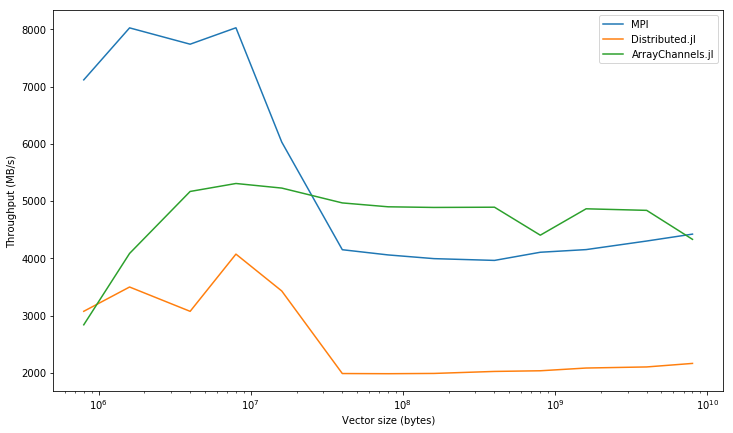
\includegraphics[width=\linewidth]{figs/pingpong.png}
	\caption{Two-process Ping-Pong performance profile}
	\label{fig:plot-pingpong}
\end{figure}

In spite of \texttt{ArrayChannels.jl} being written using Julia
serialisation constructs, we still see generally improved performance
over \texttt{Distributed.jl} for larger message sizes, due to improved
cache utilisation. The largest difference in performance is attained for
40MB messages, with 150\% improvement over \texttt{Distributed.jl}. For
messages below 100kB in size, eager message passing in
\texttt{Distributed.jl} yields improved performance due to the cost of
synchronisation in the rendezvous model outweighing the benefits of
improved access locality. For message sizes up to 16MB, MPI
significantly outperforms \texttt{ArrayChannels.jl} due its highly
optimised messaging model. Interestingly, \texttt{ArrayChannels.jl}
provides up to 18\% improved performance over MPI for message sizes
ranging between 40MB and 4GB, with deteriorating performance for 8GB
messages, while MPI performance continues to increase.

\subsection{Reduce Results}
\label{sec:reduce-results}

In the distributed reduce kernel, each process is allocated two large
vectors so that a local reduction can be performed. For our testing
purposes, each of these vectors was 8MB in size, providing 16MB to each
process. We selected these problem sizes such that in all trials with
parallel computation, the size of program memory will exceed last-level
cache, and so highlight the effects of access locality.

The reduce kernel's performance readings depicted in figure
~\ref{fig:plot-reduce} demonstrate the effect of parallelisation on
overall throughput (measured in flops per second) of the reduction
operation. In MPI, performance increases steeply with parallelisation
only for core counts above four, with only a slight increase between
three and four cores. The provision of fourteen cores in the case of MPI
provides 91\% over the sequential reading, however in both Julia
implementations (each targeting the tree topology) provide deteriorated
performance with the addition of parallelism, with fourteen cores
obtaining 84\% (with \texttt{ArrayChannels.jl}) and 46\% (with
\texttt{Distributed.jl}) of the sequential performance.

\begin{figure}[htb]
	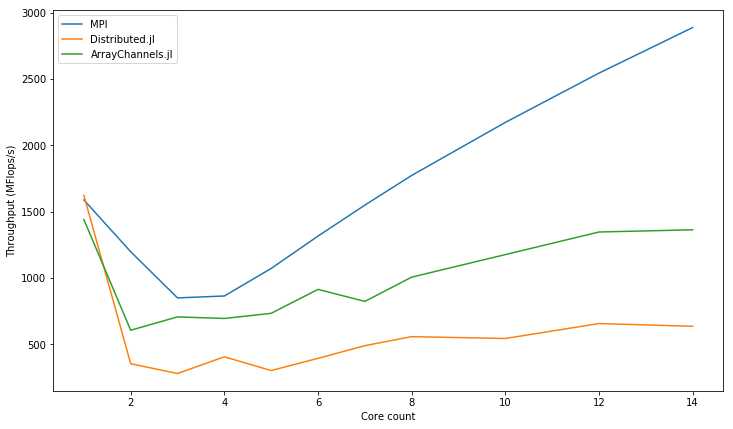
\includegraphics[width=\linewidth]{figs/reduce.png}
	\caption{Weak scaling on Distributed Reduction}
	\label{fig:plot-reduce}
\end{figure}

MPI implementations are able to target a wide variety of network
topologies in their approach to operations such as reduction, and may
even adopt different behaviour depending on the input size. By
comparison, we implement the Reduce kernel targeting exactly one
topology. In \S~\ref{sec:pingpong-results}, we observe that on a
shared-memory environment such as the testing environment, the MPI
implementation delivers far higher data throughput for 8MB messages than
either communication model in Julia. While the cost of communication in
Julia prohibits speedup due to parallelism on this kernel, this
performance degradation is mitigated by improved temporal locality in
\texttt{ArrayChannels.jl}. Performance when utilising \texttt{ArrayChannels.jl} is roughly double that of performance in \texttt{Distributed.jl}, with improvements between 68\% for 7 cores and 152\% for 3 cores.

\subsection{Transpose Results}
\label{sec:transpose-results}

In the distributed transpose kernel, all process operate on separate
portions of a large square matrix. We describe the data distribution
method in \S~\ref{sec:transpose-kernel}. Each process is allocated
2MB of this matrix, however will retain a copy of their local portion
for computation.

In figure~\ref{fig:plot-transpose}, we see that parallel performance
under Julia for the transpose kernel is greatly diminished compared to
the sequential reading and reference C-MPI code. Under
\texttt{Distributed.jl}, using parallelism obtains at most 61\% of the
sequential performance, with only 50\% under \texttt{ArrayChannels.jl}.
\texttt{Distributed.jl} obtains typically higher performance than
\texttt{ArrayChannels.jl} with execution under eight cores yielding 24\%
performance improvement.

\begin{figure}[htb]
	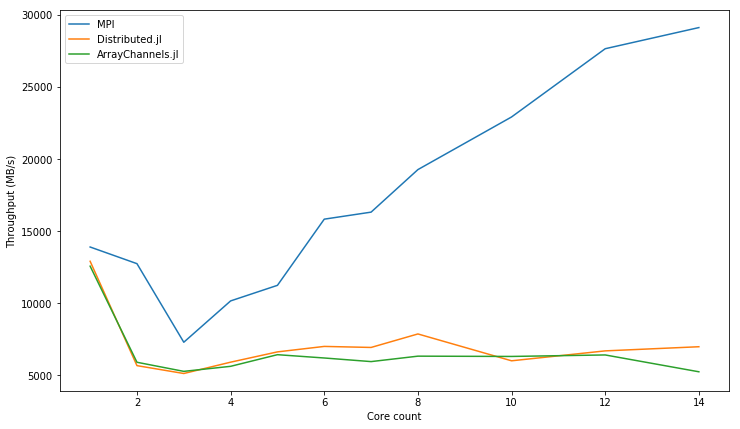
\includegraphics[width=\linewidth]{figs/transpose.png}
	\caption{Weak Scaling on Distributed Transpose}
	\label{fig:plot-transpose}
\end{figure}

As with the reduce kernel, the transpose kernel's low arithmetic
intensity and large message sizes exacerbate the weaker communication
performance in Julia compared to OpenMPI. While
\texttt{ArrayChannels.jl} is able to obtain slightly improved
performance readings over \texttt{Distributed.jl} for core-counts of two
and ten (4\% and 5\% respectively), the adopted rendezvous communication
model requires an acknowledgement of the recipient's readiness to
receive prior to communicating any data. Where individual messages are
too large, and when a large number of processes must be communicated
with, this leads to occasions where sender processes are idle when they
could instead be eagerly sending data. This leads to degraded
performance under \texttt{ArrayChannels.jl} where processes must enact
multiple communication tasks concurrently. To ensure that minimal time
is spent waiting on recipients to complete their own communication
tasks, processes may instead elect to wait on all other processes
concurrently. However, to ensure that message buffers are not
overwritten requires buffer duplication, and to facilitate this
concurrency requires increased numbers of context switches.

\subsection{Stencil Results}
\label{sec:stencil}

For the stencil kernel, we use the same problem sizes as with transpose,
and use a radius two `star' point-wise operator as depicted in figure
~\ref{fig:stencil-diagram}. As in transpose, processes must allocate a
copy of their local data for storing intermediate results during each
iteration, leading to an allocation of 4MB per process. In line with the
Intel PRK \footnote{Available at
	https://github.com/ParRes/Kernels/tree/master/MPI1.} implementation of
the stencil kernel, we attempt to distribute the source matrix into
roughly square regions subject to the factoring of the number of
processes.

As depicted in figure~\ref{fig:plot-stencil}, all three implementations feature typically increasing trends in
performance with the added parallelism, with improvements over
sequential readings of 11.0\(\times\), 4.19\(\times\) and 6.27\(\times\)
for MPI, \texttt{Distributed.jl} and \texttt{ArrayChannels.jl}
respectively. Between the two Julia implementations, we see up to 71\%
performance improvement for \texttt{ArrayChannels.jl} over
\texttt{Distributed.jl} with ten cores, with improved readings at each
core count we surveyed.

\begin{figure}[htb]
	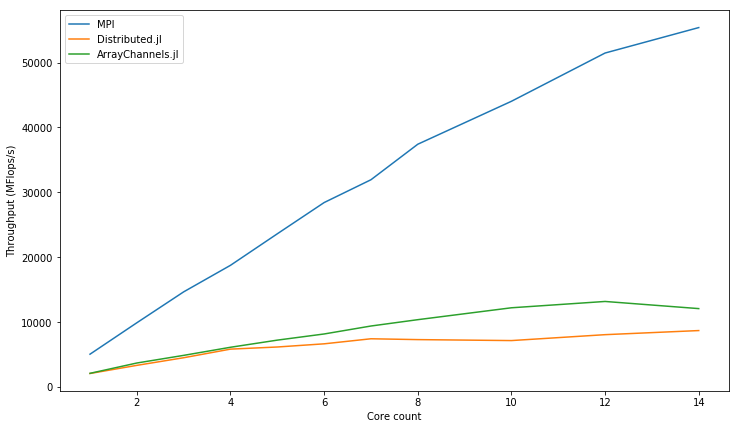
\includegraphics[width=\linewidth]{figs/stencil.png}
	\caption{Weak Scaling on Distributed Stencil}
	\label{fig:plot-stencil}
\end{figure}

In the stencil kernel, messages sizes are small compared to that of
transpose or reduce, and the arithmetic intensity is high. The ghost
regions (matrix regions that must be shared between processes) have the
potential to be stored entirely in last-level cache, and as such
\texttt{ArrayChannels.jl} provides improved performance by reissuing the
same storage location when receiving the contents of these regions at
each iteration. Communication in \texttt{Distributed.jl} will instead
generate a new buffer for each incoming message, increasing memory
latency as the memory region must be fetched into processor cache prior
to use.


\section{Conclusion}
In this article we presented the \texttt{ArrayChannels.jl} library, providing in-place communication for array data to the Julia language. The library supports a number of parallelism patterns, such as point-to-point communication, parallel reduction and the scatter / gather pattern. We evaluated the performance of both \texttt{ArrayChannels.jl} and \texttt{Distributed.jl} on a number of benchmarks to demonstrate how improved temporal locality can significantly improve the performance scalability of numerical codes.

Our evaluation revealed that while tasks involving large, overlapping communication events may still favour the eager communication model in `Distributed.jl`, however many realistic computation efforts perform better when messages are transferred in-place. By using `ArrayChannels.jl` constructs improved total throughput obtainable by message passing by up to 150\%, and on realistic benchmarks with up to 71\% for the stencil kernel and up to 152\% improvement on vector reduction.

% **************GENERATED FILE, DO NOT EDIT**************

\bibliographystyle{juliacon}
\bibliography{ref.bib}


\end{document}

% Inspired by the International Journal of Computer Applications template
